% Options for packages loaded elsewhere
\PassOptionsToPackage{unicode}{hyperref}
\PassOptionsToPackage{hyphens}{url}
\PassOptionsToPackage{dvipsnames,svgnames,x11names}{xcolor}
%
\documentclass[
  ignorenonframetext,
  aspectratio=169,
]{beamer}
\usepackage{pgfpages}
\setbeamertemplate{caption}[numbered]
\setbeamertemplate{caption label separator}{: }
\setbeamercolor{caption name}{fg=normal text.fg}
\beamertemplatenavigationsymbolshorizontal
% Prevent slide breaks in the middle of a paragraph
\widowpenalties 1 10000
\raggedbottom
\setbeamertemplate{part page}{
  \centering
  \begin{beamercolorbox}[sep=16pt,center]{part title}
    \usebeamerfont{part title}\insertpart\par
  \end{beamercolorbox}
}
\setbeamertemplate{section page}{
  \centering
  \begin{beamercolorbox}[sep=12pt,center]{part title}
    \usebeamerfont{section title}\insertsection\par
  \end{beamercolorbox}
}
\setbeamertemplate{subsection page}{
  \centering
  \begin{beamercolorbox}[sep=8pt,center]{part title}
    \usebeamerfont{subsection title}\insertsubsection\par
  \end{beamercolorbox}
}
\AtBeginPart{
  \frame{\partpage}
}
\AtBeginSection{
  \ifbibliography
  \else
    \frame{\sectionpage}
  \fi
}
\AtBeginSubsection{
  \frame{\subsectionpage}
}

\usepackage{amsmath,amssymb}
\usepackage{iftex}
\ifPDFTeX
  \usepackage[T1]{fontenc}
  \usepackage[utf8]{inputenc}
  \usepackage{textcomp} % provide euro and other symbols
\else % if luatex or xetex
  \usepackage{unicode-math}
  \defaultfontfeatures{Scale=MatchLowercase}
  \defaultfontfeatures[\rmfamily]{Ligatures=TeX,Scale=1}
\fi
\usetheme[]{Hannover}
\usecolortheme{rose}
\usepackage[]{libertinus}
\ifPDFTeX\else  
    % xetex/luatex font selection
\fi
% Use upquote if available, for straight quotes in verbatim environments
\IfFileExists{upquote.sty}{\usepackage{upquote}}{}
\IfFileExists{microtype.sty}{% use microtype if available
  \usepackage[]{microtype}
  \UseMicrotypeSet[protrusion]{basicmath} % disable protrusion for tt fonts
}{}
\makeatletter
\@ifundefined{KOMAClassName}{% if non-KOMA class
  \IfFileExists{parskip.sty}{%
    \usepackage{parskip}
  }{% else
    \setlength{\parindent}{0pt}
    \setlength{\parskip}{6pt plus 2pt minus 1pt}}
}{% if KOMA class
  \KOMAoptions{parskip=half}}
\makeatother
\usepackage{xcolor}
\newif\ifbibliography
\setlength{\emergencystretch}{3em} % prevent overfull lines
\setcounter{secnumdepth}{-\maxdimen} % remove section numbering


\providecommand{\tightlist}{%
  \setlength{\itemsep}{0pt}\setlength{\parskip}{0pt}}\usepackage{longtable,booktabs,array}
\usepackage{calc} % for calculating minipage widths
\usepackage{caption}
% Make caption package work with longtable
\makeatletter
\def\fnum@table{\tablename~\thetable}
\makeatother
\usepackage{graphicx}
\makeatletter
\def\maxwidth{\ifdim\Gin@nat@width>\linewidth\linewidth\else\Gin@nat@width\fi}
\def\maxheight{\ifdim\Gin@nat@height>\textheight\textheight\else\Gin@nat@height\fi}
\makeatother
% Scale images if necessary, so that they will not overflow the page
% margins by default, and it is still possible to overwrite the defaults
% using explicit options in \includegraphics[width, height, ...]{}
\setkeys{Gin}{width=\maxwidth,height=\maxheight,keepaspectratio}
% Set default figure placement to htbp
\makeatletter
\def\fps@figure{htbp}
\makeatother

\makeatletter
\@ifpackageloaded{caption}{}{\usepackage{caption}}
\AtBeginDocument{%
\ifdefined\contentsname
  \renewcommand*\contentsname{Table of contents}
\else
  \newcommand\contentsname{Table of contents}
\fi
\ifdefined\listfigurename
  \renewcommand*\listfigurename{List of Figures}
\else
  \newcommand\listfigurename{List of Figures}
\fi
\ifdefined\listtablename
  \renewcommand*\listtablename{List of Tables}
\else
  \newcommand\listtablename{List of Tables}
\fi
\ifdefined\figurename
  \renewcommand*\figurename{Figure}
\else
  \newcommand\figurename{Figure}
\fi
\ifdefined\tablename
  \renewcommand*\tablename{Table}
\else
  \newcommand\tablename{Table}
\fi
}
\@ifpackageloaded{float}{}{\usepackage{float}}
\floatstyle{ruled}
\@ifundefined{c@chapter}{\newfloat{codelisting}{h}{lop}}{\newfloat{codelisting}{h}{lop}[chapter]}
\floatname{codelisting}{Listing}
\newcommand*\listoflistings{\listof{codelisting}{List of Listings}}
\makeatother
\makeatletter
\makeatother
\makeatletter
\@ifpackageloaded{caption}{}{\usepackage{caption}}
\@ifpackageloaded{subcaption}{}{\usepackage{subcaption}}
\makeatother
\ifLuaTeX
  \usepackage{selnolig}  % disable illegal ligatures
\fi
\usepackage{bookmark}

\IfFileExists{xurl.sty}{\usepackage{xurl}}{} % add URL line breaks if available
\urlstyle{same} % disable monospaced font for URLs
\hypersetup{
  pdftitle={Longitudinal Design},
  pdfauthor={Usman Afzali, PhD},
  colorlinks=true,
  linkcolor={Maroon},
  filecolor={Maroon},
  citecolor={Blue},
  urlcolor={Blue},
  pdfcreator={LaTeX via pandoc}}

\title{Longitudinal Design}
\author{Usman Afzali, PhD}
\date{2024-10-07}
\logo{
\includegraphics{mds.png}}

\begin{document}
\frame{\titlepage}

\begin{frame}{Outline}
\phantomsection\label{outline}
\begin{itemize}
\tightlist
\item
  Introduction
\item
  Strengths and weaknesses
\item
  Design and analysis considerations
\item
  Types of longitudinal design
\item
  Applications and examples
\end{itemize}
\end{frame}

\begin{frame}{Introduction}
\phantomsection\label{introduction}
\begin{itemize}[<+->]
\tightlist
\item
  Measuring a variable (or variables) in the same group of subjects over
  a period of time.
\item
  Subjects are generally in the same cohort and they age together.
\item
  It is a within-subjects design (pretest-posttest)
\end{itemize}
\end{frame}

\begin{frame}
Example: Measuring IQ at 40, 60, and 80 years of age in the same cohort
(or even the same individuals).

\begin{center}
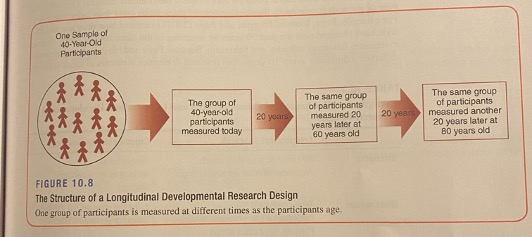
\includegraphics{figs/iq.jpg}
\end{center}
\end{frame}

\begin{frame}{Strengths}
\phantomsection\label{strengths}
\begin{itemize}[<+->]
\tightlist
\item
  Estimation of the cohort effect
\item
  Cohort effect: A cohort effect is when differences in behaviour or
  traits among people are due to the time period or events they
  experienced together, rather than their age or other factors. For
  instance, technology adoption: People born in the 1990s grew up with
  the internet and are generally more tech-savvy than those born in the
  1950s, who had to learn digital skills later in life. The difference
  in comfort with technology is a cohort effect.
\item
  Allows studying changes of behaviour in individuals across time
\end{itemize}
\end{frame}

\begin{frame}{Weaknesses}
\phantomsection\label{weaknesses}
\begin{itemize}[<+->]
\tightlist
\item
  Time consuming (for researchers and subjects), needs commitment
\item
  Very expensive
\item
  High drop-out rates (aka sample/participant attrition), that weakens
  internal validity (how?)
\end{itemize}
\end{frame}

\begin{frame}{Design and Analysis Considerations}
\phantomsection\label{design-and-analysis-considerations}
\begin{itemize}[<+->]
\tightlist
\item
  Representative sampling
\item
  Minimizing selection bias
\item
  Choosing appropriate measurement tools
\item
  Combining quantitative and qualitative approaches
\item
  Exploring inter-individual and intra-individual differences
\end{itemize}
\end{frame}

\begin{frame}{Types of Longitudinal Design}
\phantomsection\label{types-of-longitudinal-design}
\begin{itemize}
\tightlist
\item
  Trend studies
\item
  Cohort studies
\item
  Panel studies
\item
  Accelerated longitudinal designs
\end{itemize}
\end{frame}

\begin{frame}{Trend Studies}
\phantomsection\label{trend-studies}
\begin{itemize}[<+->]
\tightlist
\item
  Example: Tracking changes in cognitive abilities in a cohort of aging
  adults.
\item
  Trend studies, also known as time-trend studies, involve studying
  changes in a \textbf{single variable or phenomenon across different
  time points}. In trend studies, researchers collect data from
  different cross-sectional samples at various time intervals. The focus
  is on observing how the variable of interest changes over time within
  each sample, without necessarily tracking the same individuals across
  time.
\end{itemize}
\end{frame}

\begin{frame}{Cohort Studies}
\phantomsection\label{cohort-studies}
\begin{itemize}[<+->]
\tightlist
\item
  Example: Comparing social attitudes in different generations.
\item
  Cohort studies involve tracking \textbf{specific groups (cohorts)} of
  individuals over time. Cohorts are usually defined by a shared
  characteristic, such as birth year or life experience. Researchers
  collect data from the same group of individuals at multiple time
  points to study changes and developments within that specific cohort.
  This design allows for the examination of cohort-specific effects and
  trends.
\end{itemize}
\end{frame}

\begin{frame}{Panel Studies}
\phantomsection\label{panel-studies}
\begin{itemize}[<+->]
\tightlist
\item
  Example: Tracking academic performance in a group of students from
  childhood to adulthood
\item
  Panel studies involve collecting data from the \textbf{same
  individuals} (the panel) at multiple time points. The goal is to track
  individual trajectories and changes over time. Panel studies require
  the same participants to be measured on the same variables repeatedly,
  making them well-suited for examining within-person variability and
  changes within specific individuals over time.
\end{itemize}
\end{frame}

\begin{frame}{Accelerated Longitudinal Design}
\phantomsection\label{accelerated-longitudinal-design}
\begin{itemize}[<+->]
\tightlist
\item
  Example: Studying language acquisition in children over a few months
\item
  Accelerated longitudinal designs involve \textbf{intensive data
  collection over a shorter period} compared to traditional longitudinal
  studies. This design is particularly useful when researchers are
  interested in studying rapid changes or development within a
  relatively compressed time-frame. Accelerated designs can involve
  repeated measurements over weeks or months, capturing significant
  changes in a short span.
\end{itemize}
\end{frame}

\begin{frame}{Key Differences}
\phantomsection\label{key-differences}
\begin{enumerate}[<+->]
\item
  \textbf{Focus and Purpose}: Trend studies focus on tracking changes in
  a single variable across different samples over time, while cohort
  studies focus on specific birth cohorts or groups, panel studies track
  the same individuals, and accelerated designs focus on capturing rapid
  changes.
\item
  \textbf{Sampling}: Trend studies involve different cross-sectional
  samples at each time point, cohort studies follow specific groups,
  panel studies involve the same individuals, and accelerated designs
  may involve a focused sample over a short period.
\end{enumerate}
\end{frame}

\begin{frame}{Key Differences}
\phantomsection\label{key-differences-1}
\begin{enumerate}[<+->]
\setcounter{enumi}{2}
\item
  \textbf{Data collection}: Trend studies collect data from different
  samples at different times, cohort studies collect data from the same
  cohort over time, panel studies repeatedly measure the same
  individuals, and accelerated designs gather intensive data in a
  shorter duration.
\item
  \textbf{Research questions}: Trend studies are good for examining
  overall trends, cohort studies are useful for cohort-specific effects,
  panel studies can explore within-person changes, and accelerated
  designs capture rapid changes or developments.
\end{enumerate}
\end{frame}

\begin{frame}{Key Differences}
\phantomsection\label{key-differences-2}
\begin{enumerate}
\setcounter{enumi}{4}
\tightlist
\item
  \textbf{Benefits and challenges}: Trend studies can identify overall
  patterns but may suffer from cohort effects; cohort studies provide
  cohort-specific insights but require long-term commitment; panel
  studies allow for individual-level analysis but can be
  resource-intensive; accelerated designs capture rapid changes but may
  not capture long-term effects.
\end{enumerate}
\end{frame}

\begin{frame}{Applications of Longitudinal Studies}
\phantomsection\label{applications-of-longitudinal-studies}
\begin{itemize}[<+->]
\tightlist
\item
  \textbf{Developmental psychology}
\item
  Examining cognitive, social, and emotional development
\item
  Identifying risk and protective factors for developmental outcomes
\item
  \textbf{Clinical psychology}
\item
  Tracking treatment effectiveness and relapse prevention
\item
  Understanding trajectories of mental health disorders
\item
  \textbf{Social psychology}
\item
  Tracking changes in values, attitudes and behaviours
\end{itemize}
\end{frame}

\begin{frame}{Dunedin Multidisciplinary Health and Development Study}
\phantomsection\label{dunedin-multidisciplinary-health-and-development-study}
This study has followed a cohort of 1,037 individuals born in Dunedin,
New Zealand in 1972-1973. Participants have been assessed at various
ages to understand the development of physical health, mental health,
and social behavior over their lives. The study has provided insights
into the development of mental disorders, addiction, and antisocial
behavior.

\url{https://dunedinstudy.otago.ac.nz}
\end{frame}

\begin{frame}{The New Zealand Attitudes and Values Study (NZAVS)}
\phantomsection\label{the-new-zealand-attitudes-and-values-study-nzavs}

\includegraphics{figs/sponsors.png}
\end{frame}

\begin{frame}
The New Zealand Attitudes and Values Study (NZAVS) is a longitudinal
quantitative panel research project that began in 2009 by Prof Chris
Sibley (The University of Auckland). It focuses on investigating the
attitudes, values, and beliefs of New Zealanders over time. The study
aims to provide a comprehensive understanding of how various factors,
including demographics, experiences, and historical context, shape
individuals' opinions and behaviours.
\end{frame}

\begin{frame}
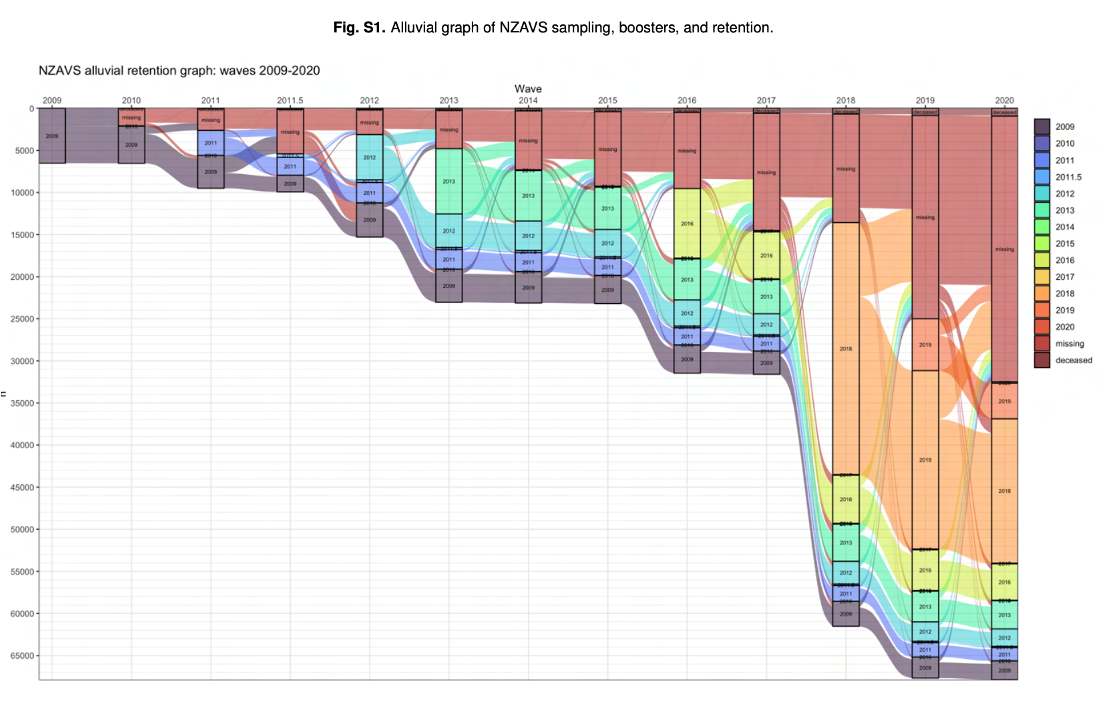
\includegraphics{figs/alluvial.png}
\end{frame}

\begin{frame}{NZAVS Features}
\phantomsection\label{nzavs-features}
\begin{itemize}[<+->]
\tightlist
\item
  \textbf{Longitudinal Nature:} The NZAVS follows a large and diverse
  sample of New Zealanders across different age groups over an extended
  period. This longitudinal design enables researchers to track changes
  in attitudes and values across generations and identify trends and
  shifts over time.
\item
  \textbf{Wide Range of Topics:} The study covers a broad range of
  topics, including social, political, environmental, and cultural
  attitudes. It delves into issues such as discrimination, social
  cohesion, well-being, environmental concerns, political participation,
  and national identity.
\item
  \textbf{Data Collection Methods:} The NZAVS collects data through
  online or printed surveys. The surveys include both established
  measures and new items designed to capture emerging issues and trends.
\end{itemize}
\end{frame}

\begin{frame}
\begin{itemize}[<+->]
\tightlist
\item
  \textbf{Public Engagement:} The study emphasizes public engagement and
  transparency. Researchers share findings with the public and
  policymakers, contributing to informed discussions and evidence-based
  decision-making.
\item
  \textbf{Treatment:} Treatments can happen -- but mostly in the form of
  natural or man-made events (e.g., changes in the government, some
  government policies/legislations, Covid-19, earthquakes, floods,
  massacres).
\end{itemize}
\end{frame}

\begin{frame}{Examples of Research Topics Addressed by NZAVS}
\phantomsection\label{examples-of-research-topics-addressed-by-nzavs}
\end{frame}

\begin{frame}{Comparing Warmth for Different Groups}
\phantomsection\label{comparing-warmth-for-different-groups}
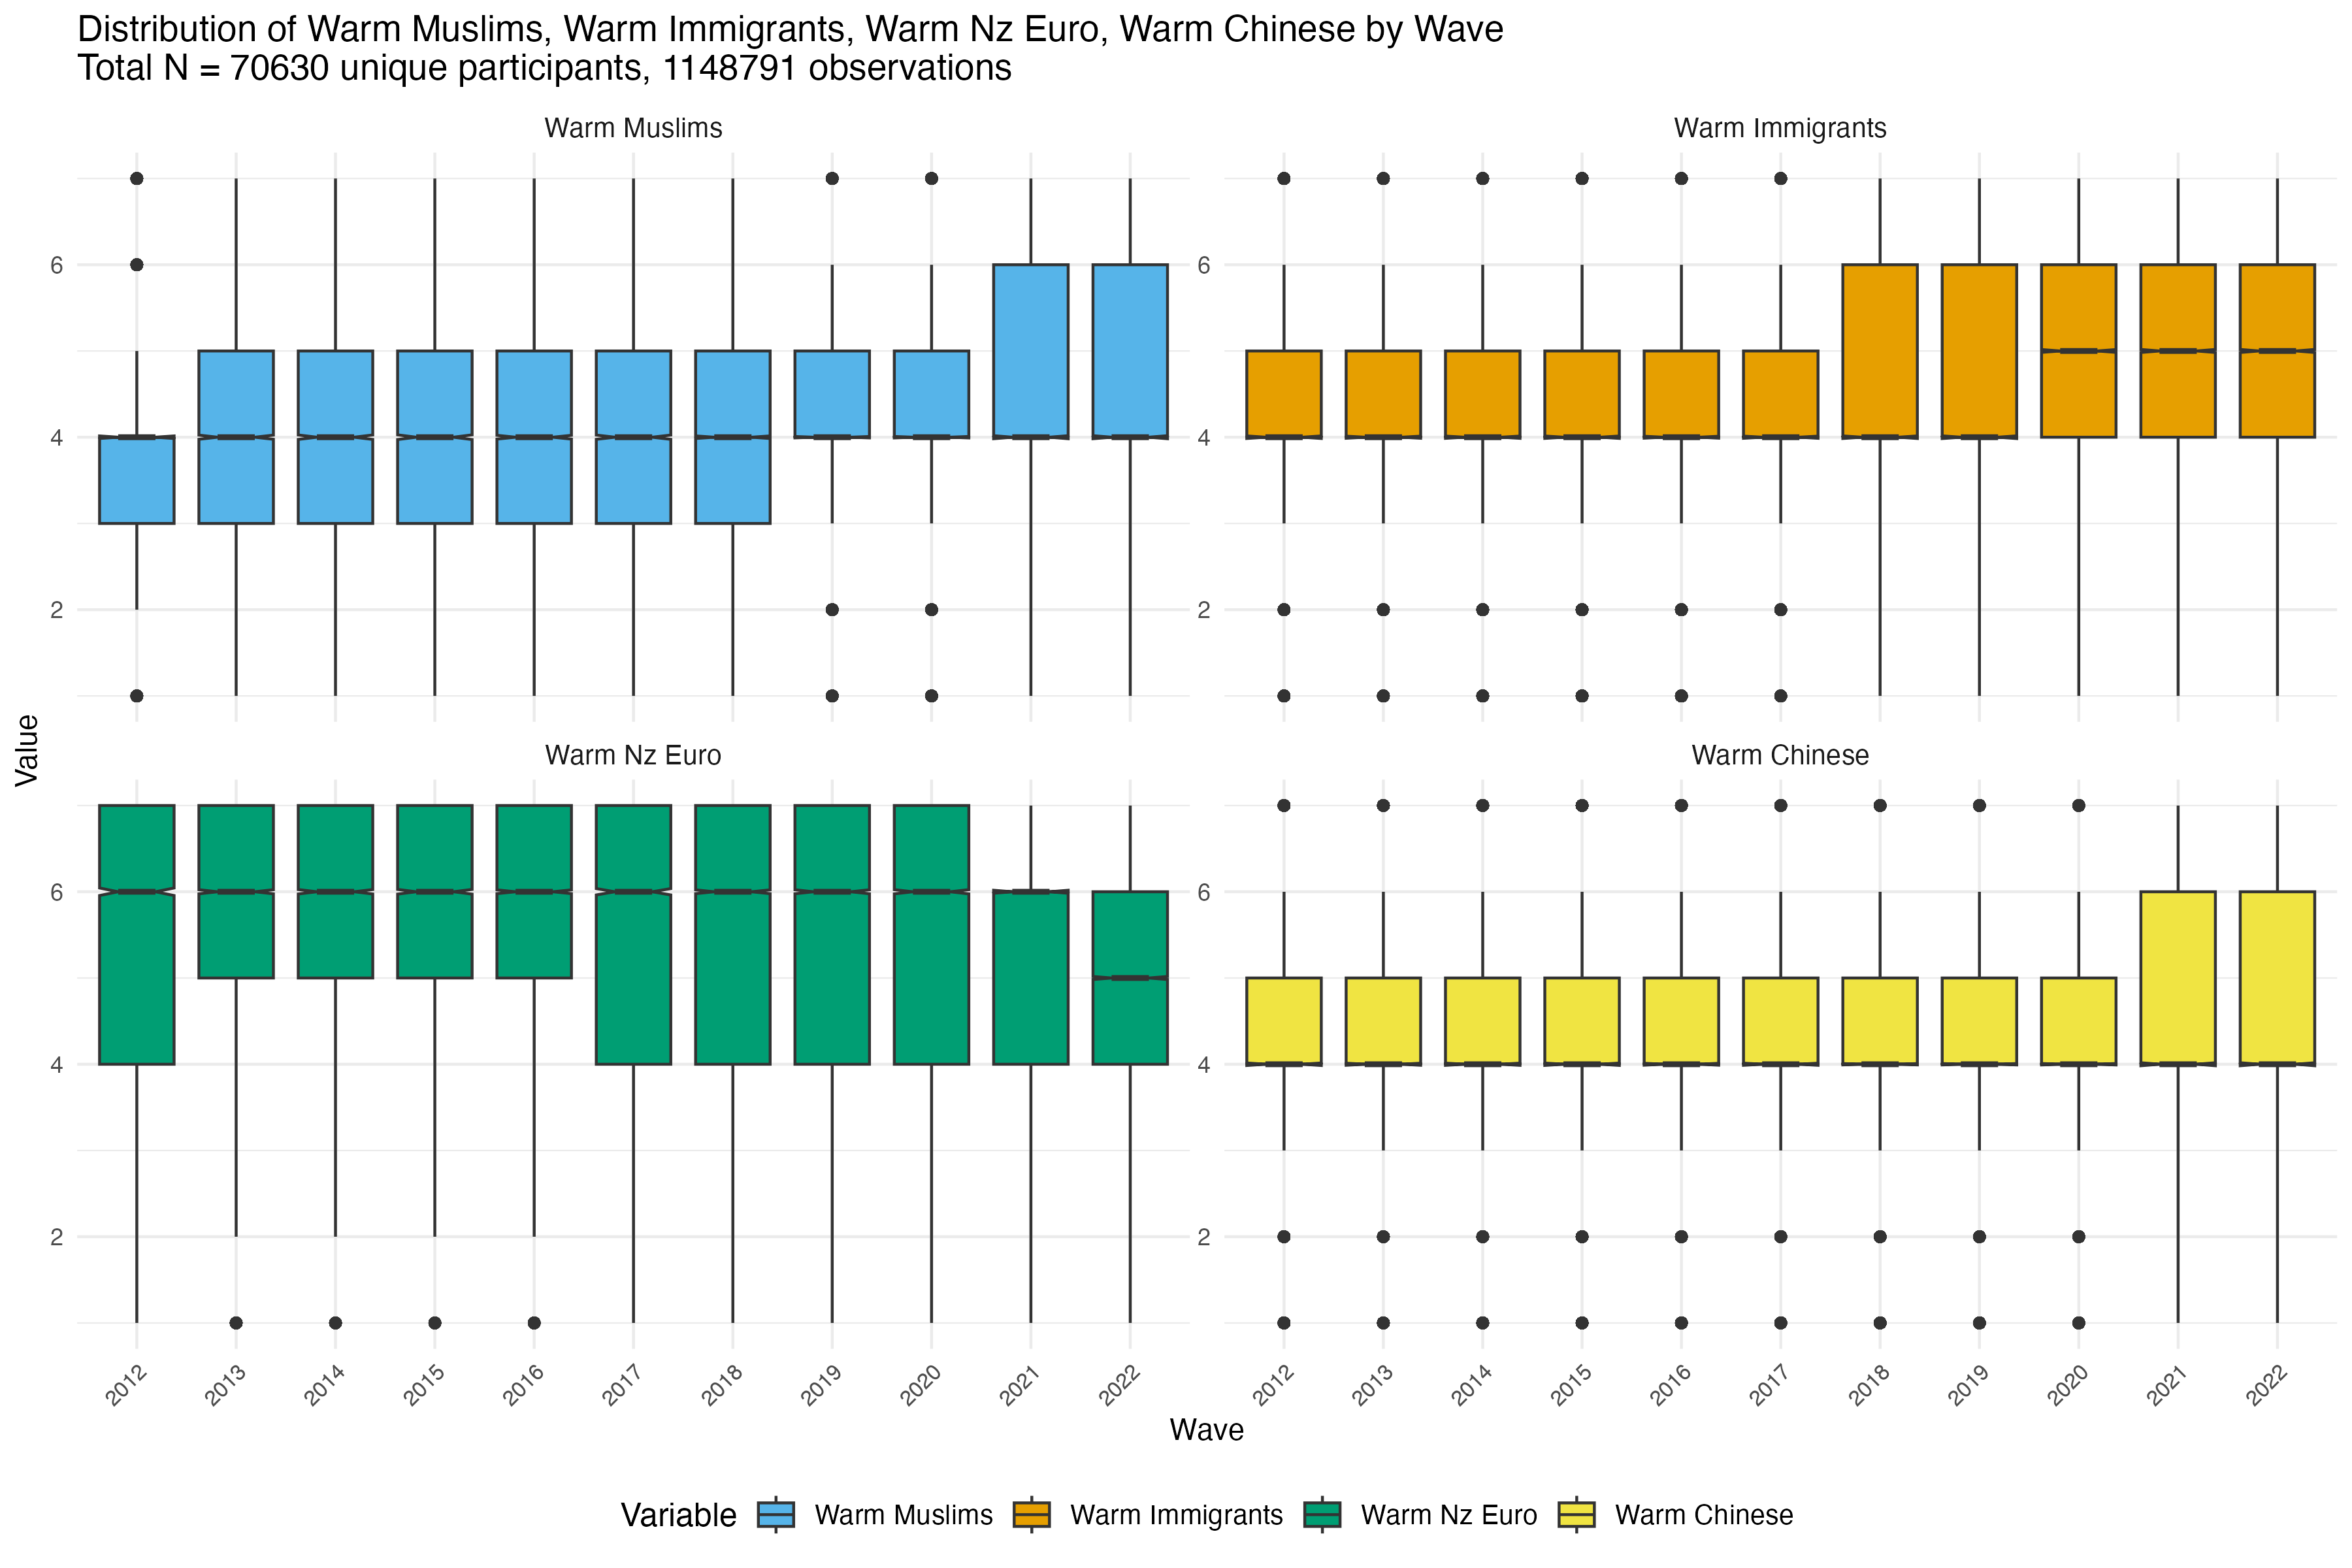
\includegraphics[width=0.85\textwidth,height=\textheight]{figs/image002.png}
\end{frame}

\begin{frame}{Overtime Change in Warth Towards Muslims}
\phantomsection\label{overtime-change-in-warth-towards-muslims}
\includegraphics[width=0.85\textwidth,height=\textheight]{figs/discontinuity_plot_warm_muslims_20240913.png}
\end{frame}

\begin{frame}{Tracking Changes Overtime}
\phantomsection\label{tracking-changes-overtime}
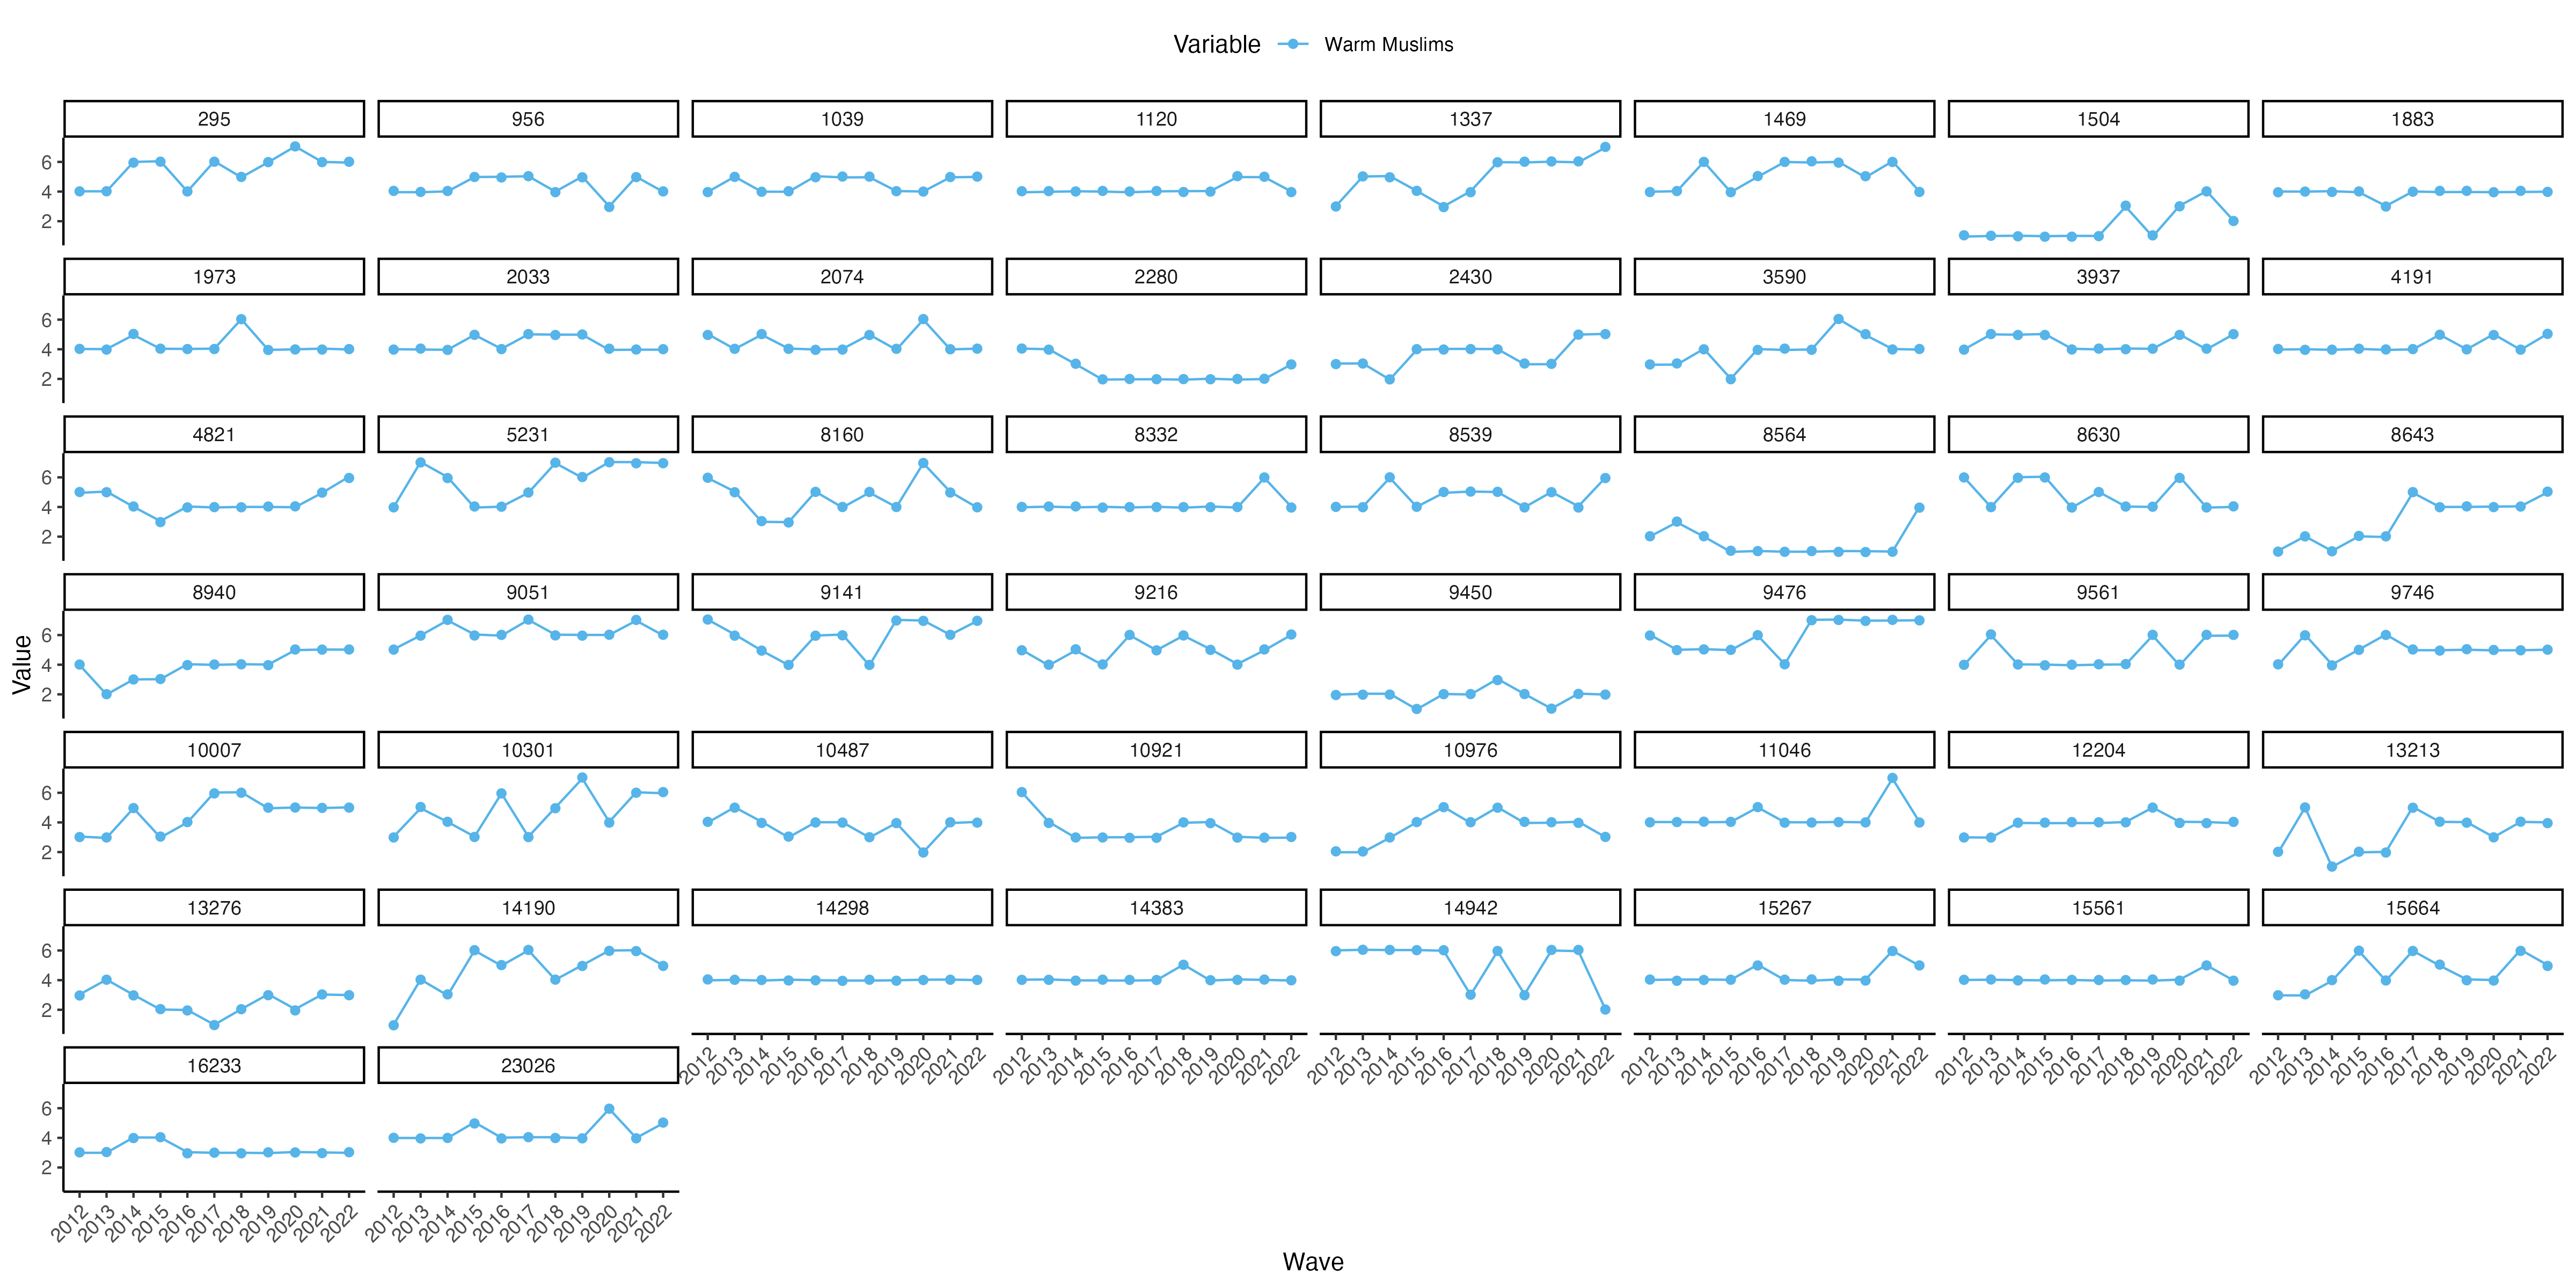
\includegraphics{figs/seed.png}
\end{frame}

\begin{frame}{NZAVS Links}
\phantomsection\label{nzavs-links}
\begin{itemize}
\tightlist
\item
  Homepage: \url{https://osf.io/75snb/wiki/home/}
\item
  Publications: \url{https://osf.io/75snb/wiki/Publications/}
\end{itemize}
\end{frame}

\begin{frame}
\textbf{Pātai}
\end{frame}

\begin{frame}
\textbf{Ka Kite}
\end{frame}



\end{document}
